%% LyX 2.3.5.2 created this file.  For more info, see http://www.lyx.org/.
%% Do not edit unless you really know what you are doing.
\documentclass[english,journal]{svproc}
\PassOptionsToPackage{natbib=true}{biblatex}
\usepackage[T1]{fontenc}
\setcounter{tocdepth}{3}
\usepackage{color}
\usepackage{babel}
\usepackage{array}
\usepackage{float}
\usepackage{booktabs}
\usepackage{textcomp}
\usepackage{multirow}
\usepackage{graphicx}
\usepackage[unicode=true,
 bookmarks=true,bookmarksnumbered=true,bookmarksopen=true,bookmarksopenlevel=1,
 breaklinks=false,pdfborder={0 0 0},pdfborderstyle={},backref=false,colorlinks=false]
 {hyperref}
\hypersetup{pdftitle={Your Title},
 pdfauthor={Your Name},
 pdfpagelayout=OneColumn, pdfnewwindow=true, pdfstartview=XYZ, plainpages=false}

\makeatletter

%%%%%%%%%%%%%%%%%%%%%%%%%%%%%% LyX specific LaTeX commands.
%% Because html converters don't know tabularnewline
\providecommand{\tabularnewline}{\\}

%%%%%%%%%%%%%%%%%%%%%%%%%%%%%% User specified LaTeX commands.
% for subfigures/subtables
\usepackage[multiple]{footmisc}
\usepackage[caption=false,font=footnotesize]{subfig}
\usepackage{diagbox}
\usepackage{array}
\usepackage{listings}
\usepackage{color}
\definecolor{lightgray}{RGB}{246,246,246}
\definecolor{darkgray}{RGB}{128,128,128}

\makeatother

\usepackage{listings}
\lstset{breaklines=true,
captionpos=b,
aboveskip=3mm,
belowskip=3mm,
showstringspaces=false,
columns=flexible,
basicstyle={\scriptsize\ttfamily},
breakatwhitespace=true,
numbers=left,
numberstyle={\scriptsize\ttfamily},
xleftmargin={0.7cm},
framexleftmargin={0.7em},
numbersep=8pt,
tabsize=3,
backgroundcolor={\color{lightgray}},
commentstyle={\color{darkgray}}}
\usepackage[bibstyle=ieee,citestyle=numeric,backend=bibtex]{biblatex}
\addbibresource{References.bib}
\begin{document}
\title{Automatic Classification of Plutonic Rocks with Machine Learning Applied to Extracted Shades and Colors on iOS Devices}
\titlerunning{Automatic Classification of Plutonic Rocks with Machine Learning}
\authorrunning{Alf\'{e}rez et al.}  
\author{
	Germ\'{a}n H. Alf\'{e}rez\inst{1},
	Sarah Hern\'{a}ndez Serrano\inst{1}, 
	Ana Mar\'{i}a Mart\'{i}nez Ardila\inst{2},
	Benjamin L. Clausen\inst{3}}
\institute{
	Facultad de Ingenier\'{i}a y Tecnolog\'{i}a, Universidad de Montemorelos, Av. Libertad 1300 Poniente, Barrio Matamoros, 67530, Montemorelos, N.L., Mexico
\email{harveyalferez@um.edu.mx}, \email{1170469@alumno.um.edu.mx} \and
	Department of Earth and Biological Sciences, Loma Linda University, Griggs Hall, 11065 Campus Street, Loma Linda, CA, 92350, USA
\linebreak
\email{anmartinez@llu.edu}\and
	Geoscience Research Institute, 11060 Campus Street, Loma Linda, CA, 92350, USA
\email{bclausen@llu.edu}
}
\maketitle
\begin{abstract}
Lightness and color are properties used for the classification of
plutonic rocks but are difficult to describe because they depend on
the experience of the observer. Moreover, the classification of plutonic
rocks using various instrumental techniques tend to be expensive and
time-consuming. To face this situation, we extracted dominant shades
and colors from 283 plutonic rock images in RGB and CIELAB formats
to train several machine learning models. The best model was deployed
on an iOS application that classifies four classes of plutonic rocks
from darkest to lightest: gabbro, diorite, granodiorite, and granite.
The best results were for the K-Nearest Neighbors model using CIELAB
dominant colors data with accuracy, precision, recall, and F-score
of 93\%.\keywords{Plutonic Rock Classification, Feature Extraction, Dominant Colors, Machine Learning, iOS Application}
\end{abstract}

\section{Introduction}

Plutonic rocks are formed when magma cools and solidifies below the
Earth\textquoteright s surface. Lightness and color are properties
used for the classification of these rocks. Color changes in rocks
may indicate changes in other rock properties (mineral assemblage,
texture, organic carbon content, and more), that is why color is a
key property for rock classification. However, these attributes are
difficult to describe because perceived shades and colors in rocks
depend on the experience of the observer \citep{NRCS-2012}. Moreover,
the instruments for accurate rock classification are time-consuming
and expensive making it prohibitive for geology students and amateurs.

Our contribution in this research work is to extract dominant shades
and colors from plutonic rock images to train several machine learning
algorithms and deploy the best model on an iOS application for the
automatic classification of four classes of plutonic rocks: gabbro,
diorite, granodiorite, and granite. No such application exists. A
mobile application offers the flexibility to carry out the classification
in real time and could be an alternative to expensive traditional
methods of rock classification.

Specifically, our three objectives are as follows:
\begin{itemize}
\item Determine the best \textit{k} number of clusters to use in the K-means
algorithm to extract the dominant colors in terms of RGB and CIELAB
color spaces from 283 images of plutonic rocks.
\item Use the extracted dominant colors and their percentage of pixels in
the images to train the following machine learning algorithms: a Convolutional
Neural Network (CNN), Decision Trees (DT), K-Nearest Neighbors (KNN),
Logistic Regression (LR), and Support Vector Machines (SVM).
\item Validate the generated models and deploy the best model in an iOS
mobile application.
\end{itemize}
This article is organized as follows: Section 2 introduces the underpinnings
of our approach. Section 3 presents the state-of-the-art of mineral
and rock classification with machine learning. Section 4 describes
the methodology. Section 5 presents and discusses the results. Finally,
Section 6 presents the conclusions and future work.

\section{Underpinnings of our Approach}

Our approach is based on the following concepts \textit{\emph{(see
Fig. }}\ref{fig:Underpinnings-of-our}).

\begin{figure}[h]
\centering{}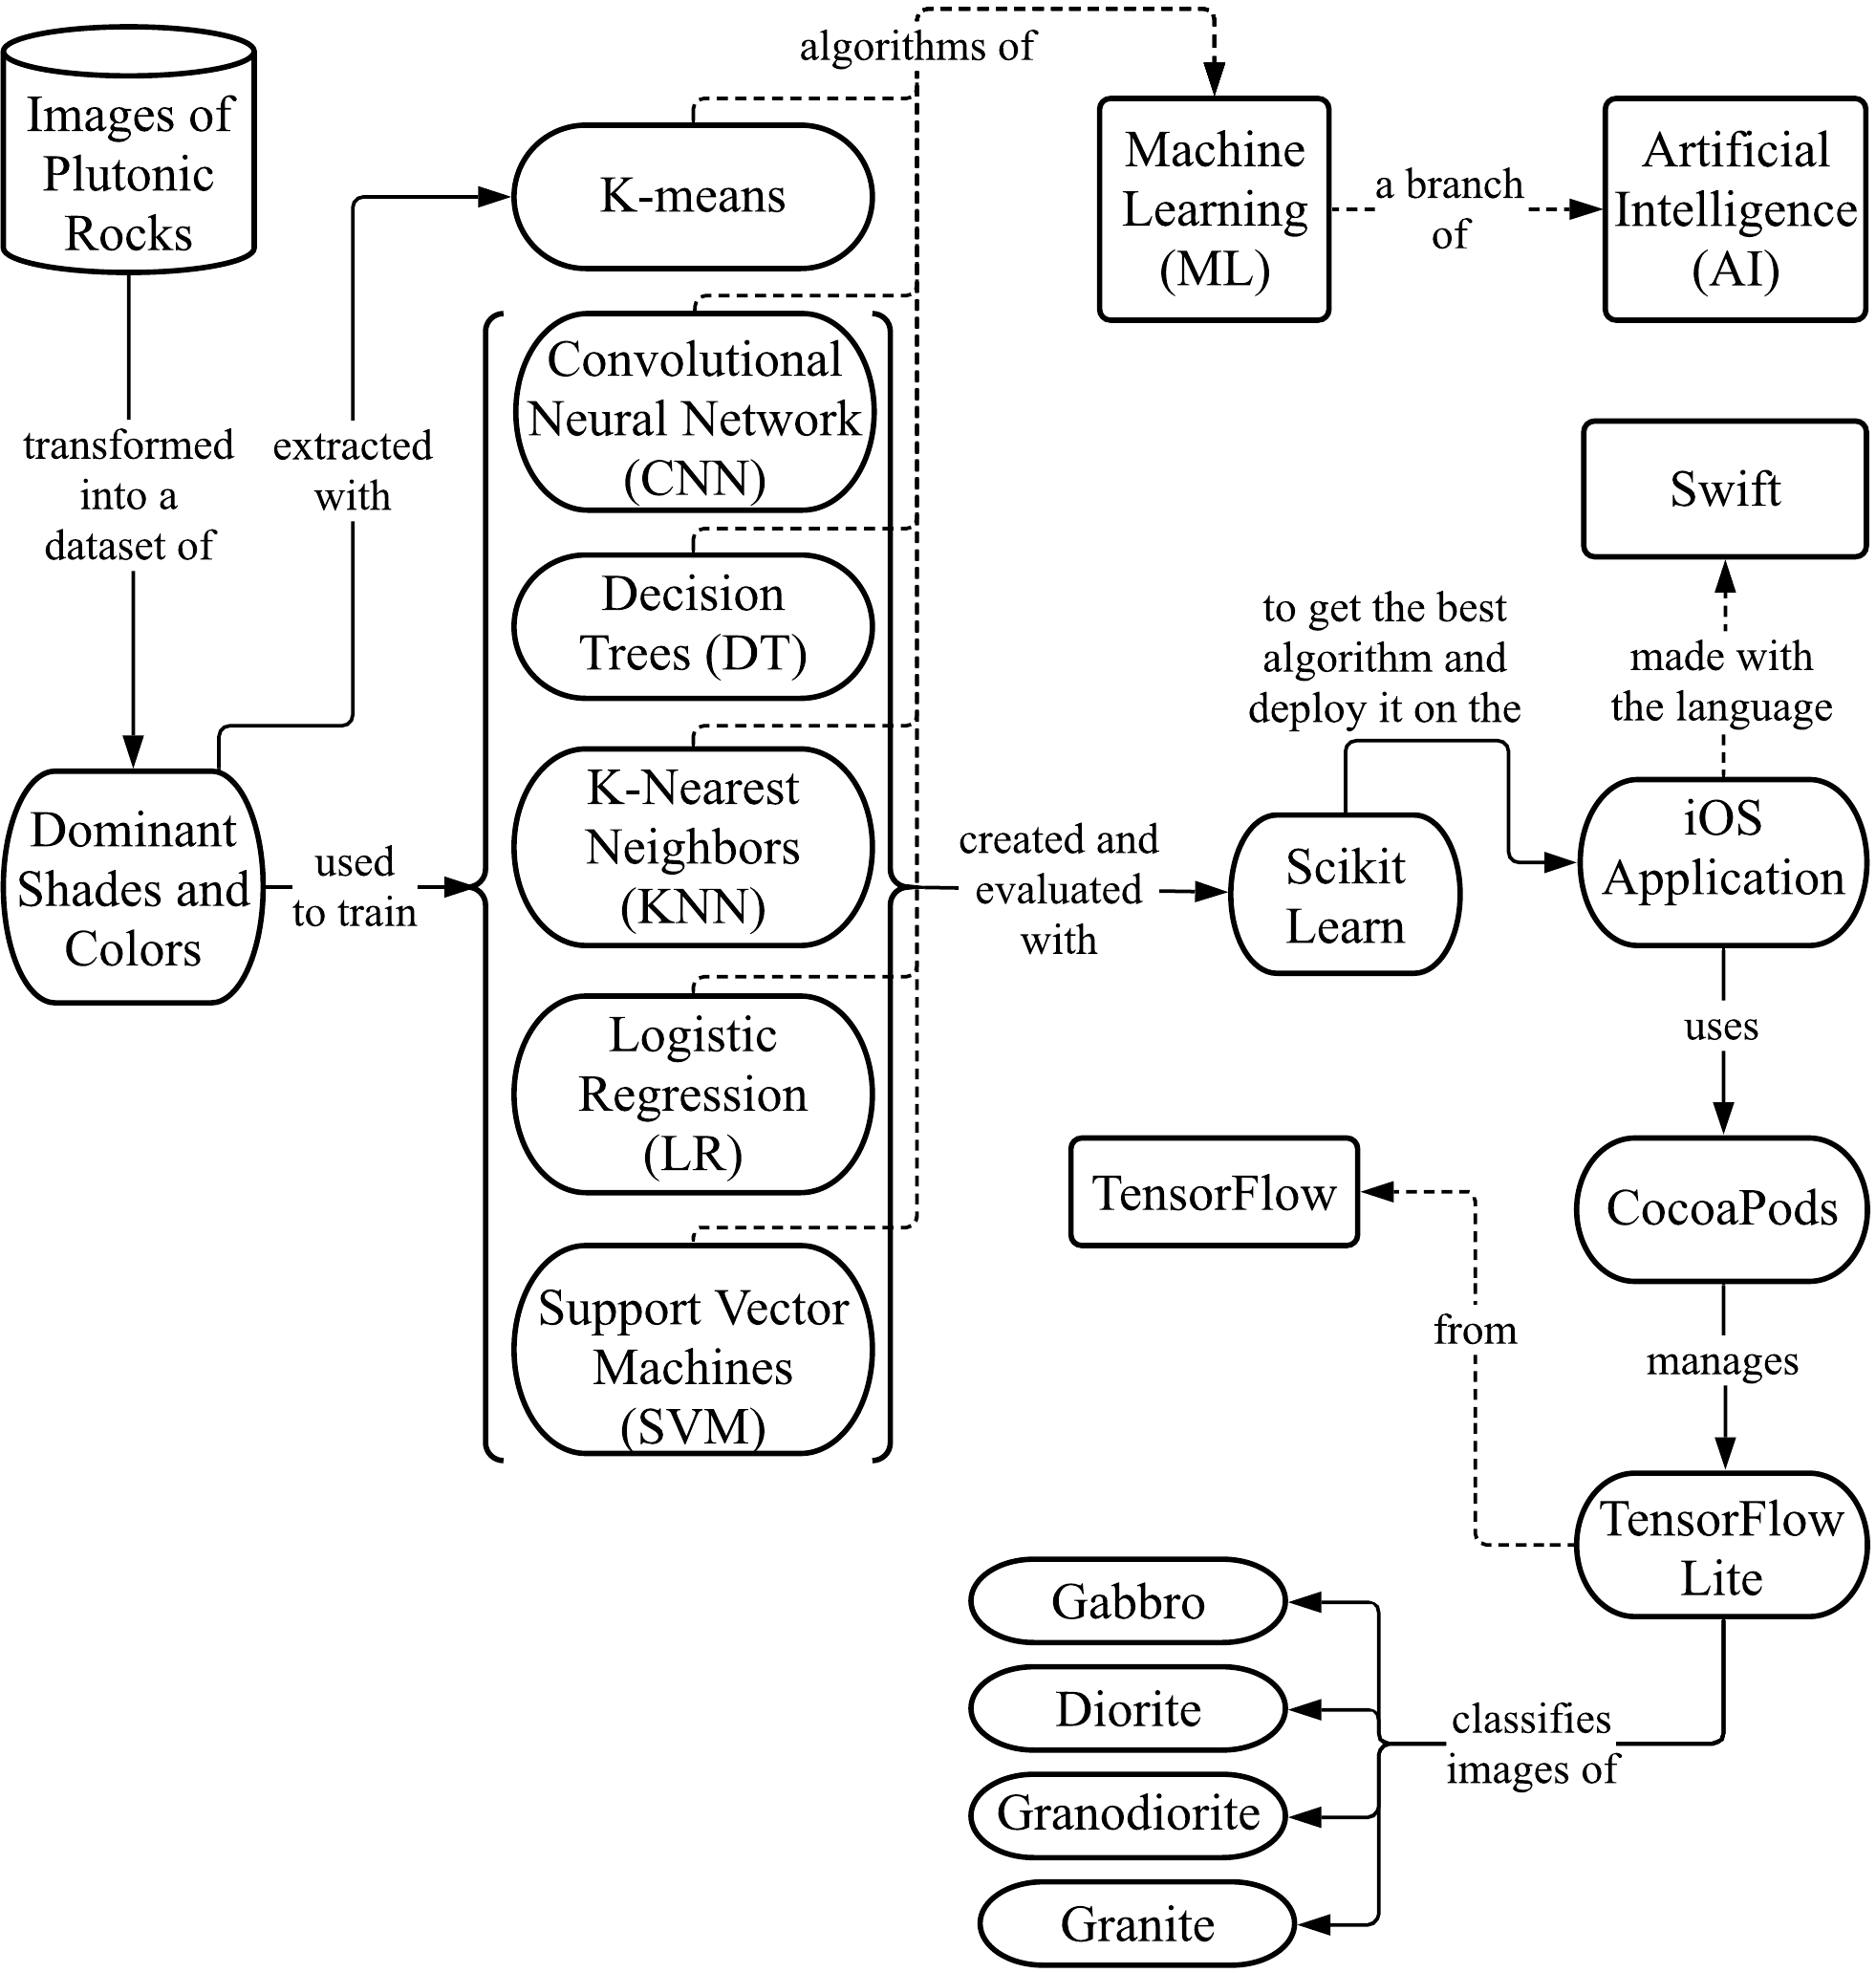
\includegraphics[height=0.4\textheight]{Figures/Underpinnings_of_our_approach}\caption{Underpinnings of our approach \label{fig:Underpinnings-of-our}}
\end{figure}


\subsection{Plutonic rocks}

Plutonic rocks crystalize inside the Earth\textquoteright s crust
from magma are generally coarse-grained and compositionally classified
by the proportion of minerals in it. According to \citep{RACEFEN-gg}:
\begin{itemize}
\item Gabbro is a plutonic rock composed mainly of calcium plagioclase and
pyroxene, with or without olivine or amphibole. It is the intrusive
equivalent of basalt and is distinguished from diorite by the nature
of plagioclase, which is higher in calcium than in sodium.
\item Diorite has about the same structural properties as granite but darker
color and more limited occurrence. Commonly it is composed of about
two-thirds plagioclase feldspar and one-third dark-coloured minerals,
such as hornblende or biotite. The presence of more sodium-rich plagioclase
and less calcium-rich plagioclase is the main distinction between
diorite and gabbro \citep{Britannica-Diorite}.
\item Granodiorite is characterized by quartz with plagioclase constituting
more than 2/3 of the total feldspars. Generally, together with granite,
it is the most abundant rock of the great batholiths. Its volcanic
equivalent is dacite. Granodiorite is similar to granite, but with
less potassium feldspar and more plagioclase, hornblende, and biotite.
\item Granite is a light-colored rock characterized by coarse to medium
crystal size, composed of approximately equal amounts of quartz, potassium
feldspar, and plagioclase as essential minerals, and smaller amounts
of other minerals, such as biotite, muscovite or hornblende.
\end{itemize}

\subsection{Machine Learning}

Machine learning is a branch of artificial intelligence that lies
at the intersection between computer science, engineering and statistics,
and often appears in other disciplines. Machine learning systems can
be classified according to the type of supervision they get during
training \citep{Harrington2012,Geron2019}. In this way, there are
two major categories:

\subsubsection{Supervised learning.}

In supervised learning, a typical task is classification. The training
set fed to the algorithm includes the desired solutions, called labels
\citep{Geron2019}. Some common supervised learning algorithms are
described as follows:
\begin{itemize}
\item Convolutional Neural Networks (CNNs) emerged from the study of the
brain\textquoteright s visual cortex. The CNN's architecture consists
of several connected layers allowing the network to concentrate on
small low-level features in the first hidden layer to assemble them
into larger higher-level features in the next layers. Their most important
building block is the convolutional layer \citep{Geron2019}.
\item Decision Trees (DT) algorithm consists of split nodes and leaf nodes.
Each split node performs a split decision and routes a data sample
either to the left or the right child node. Leaves represent the labels,
non-leaf nodes are the input features, and branches represent conjunctions
of features that lead to the classifications \citep{REINDERS201965,TAN2015493}.
\item K-Nearest Neighbors (KNN) is used to predict the label of a new point
finding a predefined number of training samples closest in distance
to that point. Being a non-parametric method, it is often successful
in classifications where the decision boundary is very irregular \citep{KNN-sklearn}.
\item Logistic Regression (LR) is commonly used to estimate the probability
that an instance belongs to a particular class. LR computes a weighted
sum of the input features (plus a bias term) and outputs the logistic
of this result. The logistic is a sigmoid function that outputs a
number between 0 and 1. This makes LR a binary classifier \citep{Geron2019}.
\item Support Vector Machines (SVM) is a powerful and versatile algorithm,
particularly well suited for classification of complex small- or medium-sized
datasets. The data is plotted in a n-dimensional space (number of
features) and a decision boundary (hyperplane) splits that space into
classes \citep{Harrington2012,Geron2019}.
\end{itemize}

\subsubsection{Unsupervised learning.}

In unsupervised learning the training data is unlabeled. K-means is
one of the most important unsupervised learning algorithms. K-means
can cluster unlabeled data very quickly and efficiently, often in
a few iterations. Its goal is to group similar instances together
into a \textit{k} number of clusters assigning each instance to one
of the clusters \citep{Geron2019}.

\subsection{Dominant colors}

The dominant colors refer to the principal colors presented in an
image. These colors are selected grouping the image pixels according
to their color in the color space (RGB or CIELAB). The colors are
represented as a three-value vector. The average color of each group
is a dominant color and its percentage is the number of pixels in
that group.

On one hand, in RGB (Red, Green, Blue) the light spectra of varying
fractions of the three primary color channels combine to make new
colors. Each channel has intensity values from 0 to 1 scaled by the
number of bits used to represent it. The 24-bit color cube used in
this research work scales the channel values in the range of 0--255.

On the other hand, CIELAB has the property of being perceptually uniform
(useful to measure the similarity between two colors) and is designed
to approximate human vision. The \textit{L} channel represents the
brightness of each pixel varying between 0 and 100. The \textit{a}
(red/green) and \textit{b} (yellow/blue) channels correspond to the
chromaticity components and contain information about the color of
a pixel, independent of its brightness. Their values vary between
-127 and 127.

\subsection{Underlying technologies}

Scikit-learn\footnote{https://www.scikit-learn.org} is a Python module
that integrates a wide range of state-of-the-art machine learning
algorithms for medium-scale supervised and unsupervised problems.
This library focuses on bringing machine learning to non-specialists
using a general-purpose high-level language. Emphasis is put on ease
of use, performance, documentation, and API consistency. It has minimal
dependencies and is distributed under the simplified Berkeley Source
Distribution (BSD) license, encouraging its use in both academic and
commercial settings \citep{scikit-learn}.

TensorFlow\footnote{https://www.tensorflow.org} is an interface for
expressing machine learning algorithms and an implementation for executing
such algorithms. A computation expressed using TensorFlow can be executed
with little or no change on a wide variety of heterogeneous systems,
ranging from mobile devices such as phones and tablets up to large-scale
distributed systems with hundreds of machines and thousands of computational
devices such as GPUs \citep{Abadi2016}.

TensorFlow Lite\footnote{https://www.tensorflow.org/lite} is a set
of tools to help developers run TensorFlow machine learning models
on mobile, embedded, and Internet of Things (IoT) devices \citep{TF-TFLite}.
TensorFlow Lite consists of two main components: The interpreter, which runs specially optimized models on many different hardware types. The converter, which converts TensorFlow models into an efficient
form for use by the interpreter, and can introduce optimizations to improve them.

Swift\footnote{https://swift.org} is an open source programming language
designed by Apple for Apple platforms and is better in type safety,
security, and hardware performance than Objective-C. Community members
actively work to port it even to more platforms like Linux \citep{Apple-Swift}.

CocoaPods\footnote{https://cocoapods.org} is a dependency manager
for Swift and Objective-C Cocoa projects. It resolves dependencies
between libraries, fetches the resulting source code, then links it
together in an Xcode workspace to build a single project \citep{CocoaPods}.

\section{Related Work}

Over the last decade, there has been considerable progress in the
application of machine learning to geochemistry \citep{Lary2018}.
In this section we present relevant research work in three areas:
image classification of rock lithology using machine learning, rock
classification with machine learning on mobile devices, and recognition
of mineral images applying machine learning and feature extraction.
Table \ref{tab:Related-work-comparison} summarizes the works presented
in this section.

\begin{table}[H]
\caption{Comparison table of the articles described in the related work \label{tab:Related-work-comparison}}

\centering{}%
\begin{tabular}{>{\centering}m{3.2em}>{\centering}m{2.2em}>{\centering}m{7.2em}>{\centering}m{4.1em}>{\centering}m{5.2em}>{\centering}m{3.6em}>{\centering}m{4.5em}>{\centering}m{6.7em}}
\toprule 
Author & Year & Dataset & Algorithm of extraction & Extracted features & Training dataset & Best model & Results\tabularnewline
\midrule
\midrule 
Fan et al. \citep{Fan2020} & 2020 & 3,208 images of 28 rock lithology categories & - & - & 80\% of the images & SqueezeNet & Accuracy: 94.55\%

File size: 9.2 MB

Execution time: 736-366 ms\tabularnewline
\midrule 
Fan et al. \citep{Fan2020a} & 2020 & 3,795 images of 30 different rock types & - & - & 80\% of the images & ShuffleNet & Accuracy: 95.30\%

File size: 18.2 MB

Execution time: 786 ms\tabularnewline
\midrule 
Ran et al. \citep{Ran2019} & 2019 & 14,589 patches from 2,290 images of 6 rock types (granite, limestone,
conglomerate, sandstone, shale, mylonite) & - & - & 60\% of the patches & 3-layer CNN & Accuracy: 97.76\%\tabularnewline
\midrule 
Zhang et al. \citep{Zhang2019} & 2019 & 481 images of 4 minerals (K-feldspar, perthite, plagioclase, and quartz) & Inception-v3 CNN model & High-level features like chromatic aberration and texture & 90\% of extracted features & Stacking model (LR, SVM, and MLP) & Accuracy: 90.9\%\tabularnewline
\midrule 
Maitre et al. \citep{Maitre2019} & 2019 & 3,192 sub-images of the views taken at different angles to a surface
with 27 mineral grain species & SLIC algorithm & Color and Peak intensity of superpixel histograms & 70\% of extracted features & Random Forest (RF) & Accuracy: 89\%\tabularnewline
\midrule 
Cheng and Guo \citep{Cheng2017} & 2017 & 4,200 images of 3 feldspar sandstone rock types (coarse, medium granular,
and fine) & - & - & 75\% of the images & 6-layer CNN & Accuracy: 98.5\%\tabularnewline
\bottomrule
\end{tabular}
\end{table}


\subsection{Image classification of rock lithology using machine learning}

In \citep{Ran2019}, Ran et al. proposed a CNN model for the classification
of six rock types (granite, limestone, conglomerate, sandstone, shale,
mylonite) and compared their results with four other common machine
learning models. A total of 2,290 images were labeled according to
the clarity of the rock and cropped into 14,589 sample patches of
512 \texttimes{} 512 pixels compressed to 128 \texttimes{} 128 pixels.
60\% of the patches of each rock type were selected for the training
dataset, 20\% for the validation dataset, and 20\% for the testing
dataset. Their proposed CNN model achieved the highest overall accuracy
of 97.76\% compared with the other models: SVM, AlexNet, GoogleLeNet
Inception v3, and VGGNet-16.

In \citep{Cheng2017}, Cheng and Guo proposed a deep CNN to identify
the granularity of feldspar sandstone rocks in images under three
color spaces: RGB, YCbCr, and HSV. A total of 4,200 images were collected
from rocks of an oil field in Ordos and divided into three types of
granularity: coarse, medium granular, and fine. The RGB images were
normalized to 224 \texttimes{} 224 pixels and converted to YCbCr and
HSV. The proposed CNN was a 6-layer structure of 4 convoluted layers
with ReLU as the activation function and 2 fully connected layers
with Softmax as the classifier. The model was trained for each color
space with 75\% of the experimental data, a batch size of 100, and
different kernel sizes and learning rates. The lowest error rates
were obtained with the learning rate of 0.0005, the kernel sizes of
11, 5, 3, and 3 for each convolutional layer respectively, and the
cross-validation for HSV color space. In RGB color space, the classification
accuracy achieved 98.5\%.

\subsection{Rock classification with machine learning on mobile devices}

In \citep{Fan2020}, Fan et al. created a method for rock lithology
recognition on Android devices based on the two lightweight SqueezeNet
and MobileNet CNNs. These models were compared with ResNet50, a heavyweight
model. The images were selected from the China Geological Survey dataset
that contains images of 28 rock categories taken by a smartphone camera.
The 3,208 images were reduced to 214 \texttimes{} 214 pixels and the
80\% of those images was used to train the two CNNs pretrained with
the ImageNet dataset. The achieved occupation sizes were 19.6, 36.8,
and 232.7 MB for MobileNet, SqueezeNet, and ResNet50. SqueezeNet was
almost two times faster than MobileNet and 7 times faster than ResNet50.
A rock recognition software based on the trained models was developed
for Android devices. The results for SqueezeNet and MobileNet on Android
smartphones were: execution time from 736 to 366 and 1,218 to 523
milliseconds, and recognition accuracies of 94.55\% and 93.27\%.

Also in \citep{Fan2020a}, Fan et al. improved their work using a
model based on ShuffleNet for quick and accurate rock lithology recognition
with smartphones and compared it with their previous work of MobileNet
and SqueezeNet. They selected 3,795 images of 30 different kinds of
rocks collected from multiple locations in East China. The ShuffleNet
model was trained using 80\% of the dataset, 3,600 iteration steps,
a learning rate of 0.008, and the parameters imported by the transfer
learning method using the ImageNet dataset. ShuffleNet occupied a
space of 18.2 MB compared to MobileNet, SqueezeNet, and ResNet50 that
occupied 34.5, 25, and 219.4 MB respectively. An Android application
was created using each model. The average recognition time for a single
rock in ShuffleNet was 786 milliseconds. It reached an accuracy of
97.65\% on a PC.

\subsection{Recognition of mineral images applying machine learning and feature
extraction}

In \citep{Zhang2019}, Zhang et al. worked on the intelligent identification
of rock-mineral images using ensemble machine learning algorithms
(model stacking). A total of 481 images of four minerals (K-feldspar,
perthite, plagioclase, and quartz) were obtained with a camera on
top of a microscope. The target RGB images were cropped to cover the
minerals and then processed to have 299 \texttimes{} 299 pixels. A
deep learning model based on Inception-v3 was adopted to extract high-level
features (such as chromatic aberration and texture) from the images
and train the algorithms of LR, SVM, KNN, Random Forest (RF), Multilayer
Perceptron (MLP), and Gaussian Naive Bayes (GNB). LR, SVM, and MLP
had a significant effect on extracted features, with higher accuracy
(90.0\%, 90.6\%, and 89.8\%) than the other models. The new features
generated by these three models were employed for the model stacking
in a new instance of LR. The stacking model showed a better performance
than the single models, with an accuracy of 90.9\%.

In \citep{Maitre2019}, Maitre et al. created several models of supervised
machine learning to recognize mineral grains in a sample surface containing
grains of 27 different mineral species (plagioclase, augite, background,
hypersthene, ilmenite, magnetite, titanite, hornblende, etc.). The
surface was scanned with an automated Scanning Electron Microscopy
(SEM). Several views of the same surface were taken with a stereo-zoom
binocular microscope to construct a large mosaic RGB image. Both images
were divided into 3,192 sub-images of 600 \texttimes{} 600 pixels.
To label the grains of the mosaic image, the simple linear iterative
clustering (SLIC) algorithm was applied for superpixel segmentation
to match each superpixel of the mosaic's sub-images with the superpixels
of the SEM's scan sub-images. From the computed RGB superpixel histograms,
the color intensity (quantile) and peak intensity (ratio between the
number of pixels in the first and second maximum bins to total number
of pixels) were extracted as features for each superpixels. KNN, RF,
and Classification and Regression Trees (CART) algorithms were trained
with 70\% of the extracted features, and tested with the other 30\%
using the kappa statistics, precision, recall, and F-score indicators.
The RF algorithm gave the best results with a global accuracy of 89\%.

\subsection{Discussion}

Machine learning has been an effective way for image classification
in geochemistry. Specifically, feature reduction was applied in \citep{Zhang2019,Maitre2019}
using deep learning and the simple linear iterative clustering (SLIC)
algorithm to extract high-level features from images of mineral samples
before training the machine learning models. Although these works
showed good results in the classification of mineral samples, the
number of extracted features was very large.

Four articles \citep{Fan2020,Fan2020a,Ran2019,Cheng2017} introduce
CNN topologies and analyze the performance of the models generated
for rock lithology classification using all the image features rather
than extracted features. The evaluation of the models showed good
results. Also, the models in the research works were trained with
diverse types of rocks instead of using only plutonic rocks. Finally,
in \citep{Fan2020,Fan2020a} the created models were deployed on an
Android mobile application for the classification of rocks. However,
there are no works presenting the deployment of machine learning for
the classification of plutonic rocks on iOS devices.

\section{Methodology}

This section describes the steps followed in this research work.

\subsection{Getting the images of the plutonic rocks}

The images of plutonic rocks were provided by the Department of Earth
and Biological Sciences at Loma Linda University. We use pictures
from plutonic rocks that were classified by using petrography and
chemistry data. Specifically, the dataset contains 283 image patches
selected from the 81 original images of four classes of plutonic rocks:
gabbro, diorite, granodiorite, and granite. In the experiments we
used clean rock samples with negligible weathering or alteration visible
to the naked eye. The images used in the following experiments were
organized in subfolders according to their class and are available
online\footnote{https://bit.ly/2P9JLEc}. Table \ref{tab:Number-of-images}
shows the number of images per class.

\begin{table}[H]
\caption{Number of images per class \label{tab:Number-of-images}}

\centering{}%
\begin{tabular}{|>{\centering}p{9em}|>{\centering}m{10em}|}
\hline 
\textbf{Class} & \textbf{Number of images}\tabularnewline
\hline 
\raggedright{}Diorite & 78\tabularnewline
\hline 
\raggedright{}Gabbro & 65\tabularnewline
\hline 
\raggedright{}Granite & 70\tabularnewline
\hline 
\raggedright{}Granodiorite & 70\tabularnewline
\hline 
\raggedright{}\textbf{Total of images} & \textbf{283}\tabularnewline
\hline 
\end{tabular}
\end{table}


\subsection{Preparing the data}

In this step, the images were processed in order to obtain the color
values of the image pixels in RGB and CIELAB color spaces.

First, all files in the subfolders were processed in RGB format and
labeled according to their container subfolder (e.g. images in the
granite subfolder are labeled as granite). Afterwards, the RGB values
of the image pixels were converted to CIELAB values using the ``rgb2lab''
function of the ``color'' class of the Scikit-image module. In this
way, it is possible to train the models in the two color spaces and
determine which color format is the most appropriate for classifying
the dominant colors of the 4 classes of plutonic rocks. The notebook
with the source code for data preparation is available online\footnote{http://bit.ly/3pyh3JL}.

\subsection{Determining the best number of color clusters}

The K-means algorithm was used to extract the dominant colors from
the images. The Elbow method was used to calculate the optimal number
of clusters \textit{k} to use by the K-means algorithm. This method
consists of iterating in a range of possible cluster numbers and determine
the best one. The \textit{k} value ranged from 2 to 20 was declared
to obtain the scores of K-means at each cluster number. Finally, we
plotted the scores with their respective \textit{k} number. The number
at the elbow in the plot indicates the best \textit{k} number of clusters,
which is 4 for this experiment \textit{\emph{(see Fig. }}\ref{fig:The-Elbow-method}).

\begin{figure}[H]
\begin{centering}
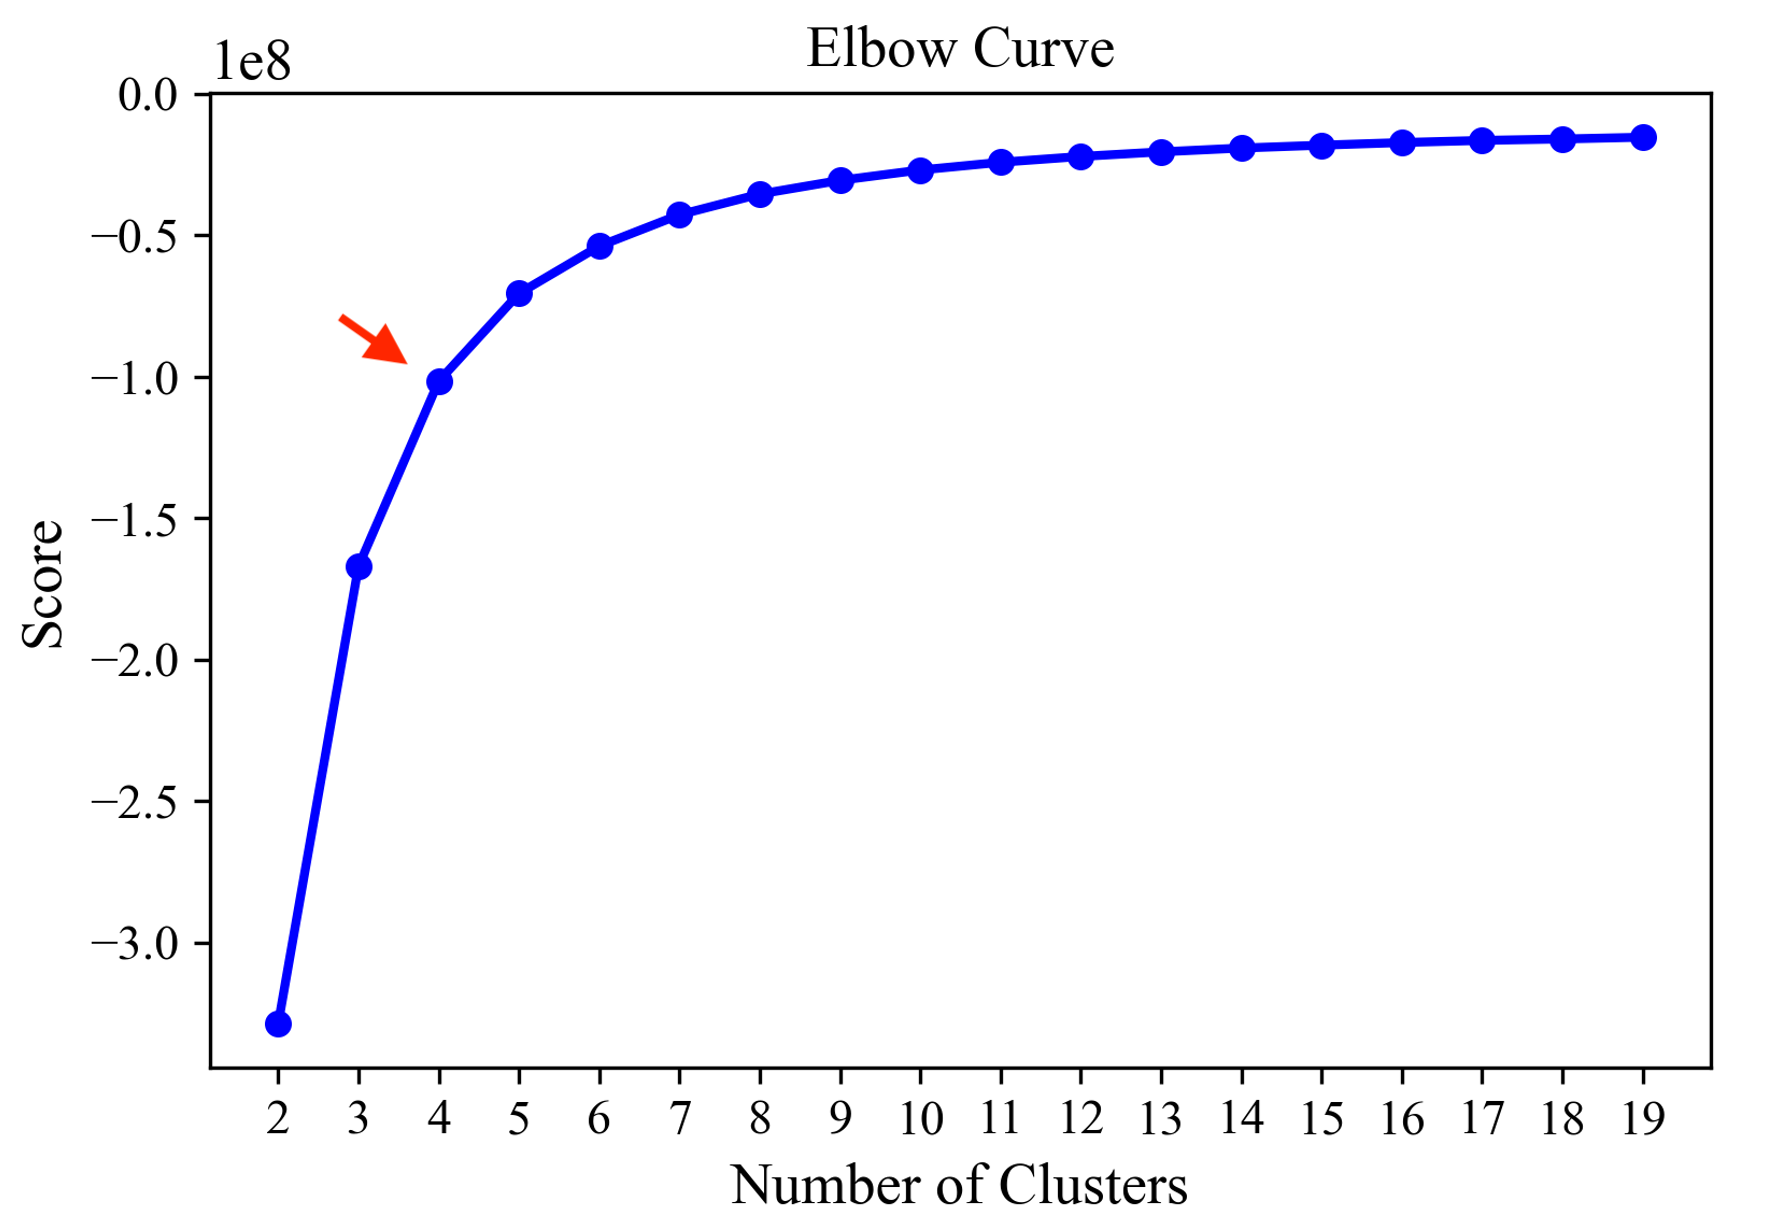
\includegraphics[width=1\textwidth]{Figures/Elbow_curve}
\par\end{centering}
\caption{The Elbow method returned the optimal \textit{k} number of clusters
\label{fig:The-Elbow-method}}
\end{figure}


\subsection{Color extraction}

In this step, the dominant colors were extracted from the rock images.
In Listing \ref{list:get-dominant-colors}, the ``get\_dominant\_colors''
function receives the pixel values of an image to train the K-means
algorithm with \textit{k} clusters. In line 6, K-means works by separating
the pixels of the image into 4 clusters of similarly colored pixels.
The colors at each cluster center reflect the average value of the
attributes of all members of a cluster. The percentage of a cluster
is the number of pixels within that color cluster and is calculated
in lines 8 to 10. Finally, the centroid of each cluster and its percentage
are sorted in increasing order of percentage and added to a features
list in lines 12 to 17. The returned list in line 19 are the sixteen
features: the four dominant colors represented by the three channels
of the selected color format and the percentage of each dominant color
(see Fig. \ref{fig:Dominant-colors-and}).

\lstinputlisting[language=Python,caption={Function to extract the dominant colors from a single image},label={list:get-dominant-colors}]{Listings/get_dominant_colors.txt}

In Listing \ref{list:iterate-to-extract-colors}, the processed data
in RGB format is iterated in lines 4 to 6 and the dominant colors
are extracted in line 5 with the function described in Listing \ref{list:get-dominant-colors}.
The colors are added to a new list of extracted colors in line 6.
This process is also made for the CIELAB data in lines 8 and 9. Finally,
the extracted colors in RGB and CIELAB formats are saved together
with their respective rock label in different CSV files. These files
were used in the next step to train the machine learning algorithms.
The CSV files with the extracted dominant colors in RGB and CIELAB
color spaces are available online\footnote{https://github.com/sarah-hs/Color-extraction/blob/main/colors\_RGB.csv}\footnote{https://github.com/sarah-hs/Color-extraction/blob/main/colors\_LAB.csv}.

\lstinputlisting[language=Python,caption={Iterate original data to extract dominant colors},label={list:iterate-to-extract-colors}]{Listings/iterate_to_extract_colors.txt}

\begin{figure}[H]
\begin{centering}
\includegraphics[height=0.73\textheight]{Figures/Extracted_colors}
\par\end{centering}
\caption{Sample rocks with their dominant colors in percentage order and their
average color\label{fig:Dominant-colors-and}}
\end{figure}


\subsection{Data normalization and label encoding}

First, in this step we loaded the dominant colors data from the CSV
files generated in the previous step. The dominant colors data are
the features loaded into \textit{x}, and the rock classes are the
labels loaded into \textit{y}. Second, in order to train and test
the models, the \textit{x} and \textit{y} data were divided into a
training set of 80\% and a test set of 20\% using the ``train\_test\_split''
function of the ``model\_selection'' class of Scikit-learn. Afterwards,
we normalized the \textit{x} data of train and test sets using the
``MinMaxScaler'' function of the ``preprocessing'' class of Scikit-learn.
This function scales each feature to a given range of 0 to 1. Finally,
we encoded the \textit{y} data in order to train the machine learning
models transforming the labels into values from 0 to 3 representing
the four rock classes of plutonic rocks: gabbro, diorite, granodiorite,
and granite respectively. The encoding process was made with the ``LabelEncoder''
function of the ``preprocessing'' class of Scikit-learn.

\subsection{Training the different algorithms with the extracted dominant colors}

The following five machine learning models were trained in this experiment
using the RGB and afterwards the CIELAB dominant colors data: DT,
KNN, LR, SVM, and a sequencial CNN topology with the following layers:
a convolutional layer (32 filters, kernel size = 2, padding = same,
input shape = 16 x 1, and activation = RELU); a max pooling layer
(pool size = 2); a convolutional layer (64 filters, kernel size =
2, padding = same, and activation = RELU); a max pooling layer (pool
size = 2); a flatten layer; and two dense layers, one with 64 filters
and RELU activation and another one with 4 filters, one per class,
and a SOFTMAX activation function. The notebooks showing the code
for training and validation of the generated models with RGB and CIELAB
data are available online\footnote{https://github.com/sarah-hs/Color-extraction/blob/main/train-RGB.ipynb}\footnote{https://github.com/sarah-hs/Color-extraction/blob/main/train-LAB.ipynb}.

\subsection{Creation of the iOS application}

The best model was exported with Tensorflow Lite and deployed in an
iOS mobile application to make the classification of images of four
classes of plutonic rocks in real time.

The main requirements to develop the application were the Xcode IDE,
the Xcode command-line tools, a valid Apple Developer ID, and the
CocoaPods dependency manager. The application was written mostly in
Swift and uses the following two libraries to perform the extraction
of the dominant colors and the rock image classification:
\begin{itemize}
\item The DominantColor\footnote{https://github.com/indragiek/DominantColor}
dependency is an open source library written in Swift. It finds the
dominant colors of an image using the K-means clustering algorithm.
\item The TensorFlowLite Swift\footnote{https://github.com/tensorflow/tensorflow/tree/master/tensorflow/lite/swift}
library is TensorFlow's lightweight solution for Swift developers.
It enables low-latency inference of on-device machine learning models
with a small binary size and fast performance supporting hardware
acceleration. For the application, TensorFlowLiteSwift pod name was
added into the project's Podfile, and from command line the library
was resolved into the Xcode project by the CocoaPods dependency manager.
\end{itemize}

\section{Results}

Table \ref{tab:Models-results} shows the average accuracy, precision,
recall, and F-score results of each model evaluated with the test
sets of dominant colors in RGB and CIELAB color formats. The models
generated with the KNN, SVM, LR, and CNN algorithms gave better results
with CIELAB data than with RGB data. The results with the DT model
were better in RGB. The best results were for the KNN model using
the CIELAB dominant colors data with an accuracy, precision, recall,
and F-score of 93\%. The training time of the KNN model was 4.33 minutes.

\begin{table}[H]
\caption{Results of the models in terms of accuracy, precision, recall, and
F-score\label{tab:Models-results}}

\centering{}%
\begin{tabular}{>{\centering}m{4em}>{\centering}m{4.7em}>{\centering}m{4.7em}>{\centering}m{4.7em}>{\centering}m{4.7em}}
\toprule 
\multirow{1}{4em}{\textbf{Model}} & \textbf{Accuracy} & \textbf{Precision} & \textbf{Recall} & \textbf{F-score}\tabularnewline
\midrule 
\multicolumn{5}{c}{with CIELAB dominant colors}\tabularnewline
\midrule 
\noindent \raggedright{}CNN & \noindent 0.81 & 0.82 & 0.82 & 0.81\tabularnewline
\midrule 
\noindent \raggedright{}DT & \noindent 0.68 & 0.68 & 0.69 & 0.68\tabularnewline
\midrule 
\noindent \raggedright{}KNN & \noindent 0.93 & 0.93 & 0.93 & 0.93\tabularnewline
\midrule 
\noindent \raggedright{}LR & \noindent 0.63 & 0.64 & 0.66 & 0.63\tabularnewline
\midrule 
\noindent \raggedright{}SVM & \noindent 0.81 & 0.82 & 0.82 & 0.80\tabularnewline
\midrule 
\multicolumn{5}{c}{with RGB dominant colors}\tabularnewline
\midrule 
\noindent \raggedright{}CNN & 0.70 & 0.72 & 0.72 & 0.71\tabularnewline
\midrule 
\noindent \raggedright{}DT & 0.72 & 0.73 & 0.72 & 0.73\tabularnewline
\midrule 
\noindent \raggedright{}KNN & 0.79 & 0.80 & 0.79 & 0.79\tabularnewline
\midrule 
\noindent \raggedright{}LR & 0.63 & 0.64 & 0.65 & 0.62\tabularnewline
\midrule 
\noindent \raggedright{}SVM & 0.53 & 0.60 & 0.49 & 0.46\tabularnewline
\bottomrule
\end{tabular}
\end{table}

Table \ref{tab:KNN-results} shows the evaluation results of the KNN
model for each rock class in terms of precision, recall, and F-score
using the CIELAB dominant colors data.

\begin{table}[H]
\caption{Results of KNN for each rock class with CIELAB data\label{tab:KNN-results}}

\centering{}%
\begin{tabular}{|>{\raggedright}p{6em}|>{\centering}p{4.7em}|>{\centering}p{4.7em}|>{\centering}p{4.7em}|}
\hline 
\multirow{1}{6em}{\textbf{Class}} & \textbf{Precision} & \textbf{Recall} & \textbf{F-score}\tabularnewline
\hline 
\raggedright{}Diorite & 0.89 & 1.00 & 0.94\tabularnewline
\hline 
\raggedright{}Gabbro & 0.93 & 1.00 & 0.96\tabularnewline
\hline 
\raggedright{}Granite & 1.00 & 0.92 & 0.96\tabularnewline
\hline 
\raggedright{}Granodiorite & 0.92 & 0.79 & 0.85\tabularnewline
\hline 
\end{tabular}
\end{table}

The KNN model was deployed on the iOS application (see Fig. \ref{fig:Application-workflow}).
There are two ways to make the classification of new rocks on this
application. The first way is taking a picture with the ``Open Camera''
button shown in step 1A of Fig. \ref{fig:Application-workflow}. When
camera opens, the new scene of step 2A appears and displays the device
camera. The second way is choosing a photo from the ``Photo Library''.
The ``Open Library'' button in step 1B opens the photo library of
the device as shown in step 2B. The extraction of the dominant colors
is performed after the image was loaded with the ``dominantColorsInImage''
function. Thereafter, the ``Classify'' button in step 3 is enabled
to classify the new rock image into: gabbro, diorite, granodiorite,
or granite. When the button is pressed the extracted colors are converted
to CIELAB and sorted in ascending order by their percentage of pixels
in the image. These colors and their percentage are used as the input
tensor for the model imported from the ``tflite'' file containing
its graph. Optionally, the dominant colors and the average colors
of the selected image can be displayed pressing the ``Extracted''
and ``Average'' buttons of steps 4A and 4B respectively.

\begin{figure}[H]
\begin{centering}
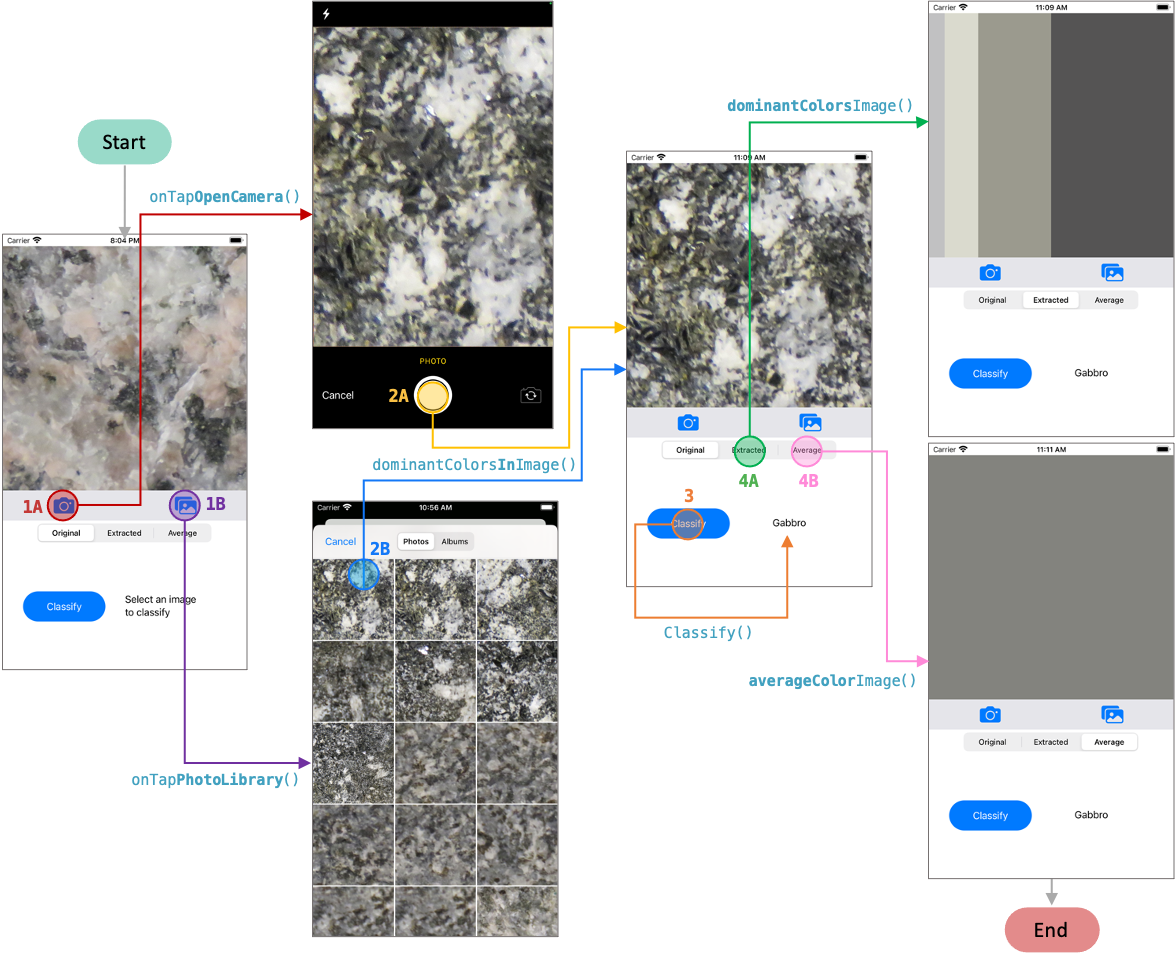
\includegraphics[width=1\textwidth]{Figures/App_workflow}
\par\end{centering}
\caption{Application workflow \label{fig:Application-workflow}}
\end{figure}

At runtime, the classification with the KNN exported model took 339.87
milliseconds. The size of the model was 0.018 MB. 

\section{Conclusions and future work}

In this research work, five machine learning algorithms were trained
with just the four dominant colors extracted from images of plutonic
rocks. The best model was found with the KNN algorithm trained with
the dominant colors in the CIELAB color format of 283 images. The
KNN model has an accuracy, precision, recall, and F-score values of
93\%.

As future work, the datasets for training and validation will be extended
with a larger number of plutonic rock images taken in the field, rather
than in the lab. Also, images will be taken under different conditions
-- different distances, angles, and lighting effects, e.g., blue
vs. cloudy sky, with weathering or alteration, shadows, vegetation,
and moss.

\printbibliography

\end{document}
